
\section{Motivation}
Empirical measurements are critical tasks to capture the effect of developers' choice on software energy consumption.
To accomplish this, one should not overlook the benchmarking pitfalls highlighted in the state of the art.
Moreover, when it comes to measuring the energy consumption of software, other obstacles arise, such as the impact of hardware, the difference between the machines used for measurements purpose and the ones that may apply the findings, etc. 
Moreover, significant improvements in computer science have resulted in an increase in the quantity of obsolete results.
It is even more difficult to address all of them in studies that compare multiple solutions.
Furthermore, there may have been the appearance of new candidates, as well as the development of others between the preliminary experiment and the published results.
As a result, it is not only required to ensure the "reproducibility" of the results, but also to make way for new candidates.
Hence, we would like to propose a new concept to leverage experiments, which we call "Extension".
The capacity to provide the tools required not only to repeat the experiments, but also to include additional candidates, workloads, or relevant key performance indicators.

This chapter discusses how to adapt the state-of-the-art of empirical analysis in the energy consumption field, highlighting the difficulties and the various techniques to overcome them. 

%% this is might be the part that treats reproducibility for my case 



%%%%%%%%% preliminary taughts and section structure 
% The need of reproducibility in our field - software optimization based on empirical studies -

% The importance of Virtualisation for reproducibility \cite{howe_virtual_2012}
% some of the most important parts are
% - fewer constraints on research methods
% - on-demand backups
% - virtual Machines as Publications
% - more Variables captured



%%%% part of the state of the art 
% In the area covered by this PhD thesis, reproducibility might be achieved by ensuring the same execution settings of physical nodes, virtual machines, clusters or cloud environments.
%%% why it won't work for energy consumption 
% However, when it comes to measuring the energy consumption of a system, applying acknowledged guidelines and carefully repeating the same benchmark can nonetheless lead to different energy footprints not only among homogeneous nodes, but even within a single node.
%% reseasons why 
% One major problem that hinders the reproducibility of the empirical benchmarks is the interaction with the external environment, either as concurrency or dependencies.
% Therefore, researchers cannot observe the same results, unless they duplicate the same environment.


\subsection{Extension}
We propose to extend the benchmarking framework suggested by the \emph{Collaboratory on Experimental Evaluation of Software and Systems in Computer Science}\footnote{\url{http://evaluate.inf.usi.ch/}} to address those limitations.
Instead of only presenting the four primary aspects of their guidelines that were mentioned in state of the art~\cref{sec:soa_reproducibility}, we propose an abstract model to describe an empirical experiment:

\emph{context}: the hardware and the software configuration for the actual experiment, the purpose of this part is to provide extra information to help readers have a better judgement on the results and to be able reproduce the experiment while diminishing the impact of the external factor . 
An \emph{orchestrator} which its job to run the experiment. 
The orchestrator provides three interfaces: 

Workload interface  : Wich provides a set of functions that should be implemented by the workload  
Candidate interface : 
Observer interface : provides a set of metrics that are collected by the orchestrator during the expermentation. note that some of those metrics are external, such the energy consumption of the system , execution time, execution stack ..etc . 


% \begin{itemize}
%     \item textbf{expermimental protocol}: Which describes, the context and  an orchestrator that handles the experiment, this orchestrator should take as an entry 
%     \item \textbf{candidates}: a set of candidates that will be used in the experiment. The candidates should be agnostic of the experiment context and they all
% \end{itemize}

% \begin{figure}%[!htb]
%     \center{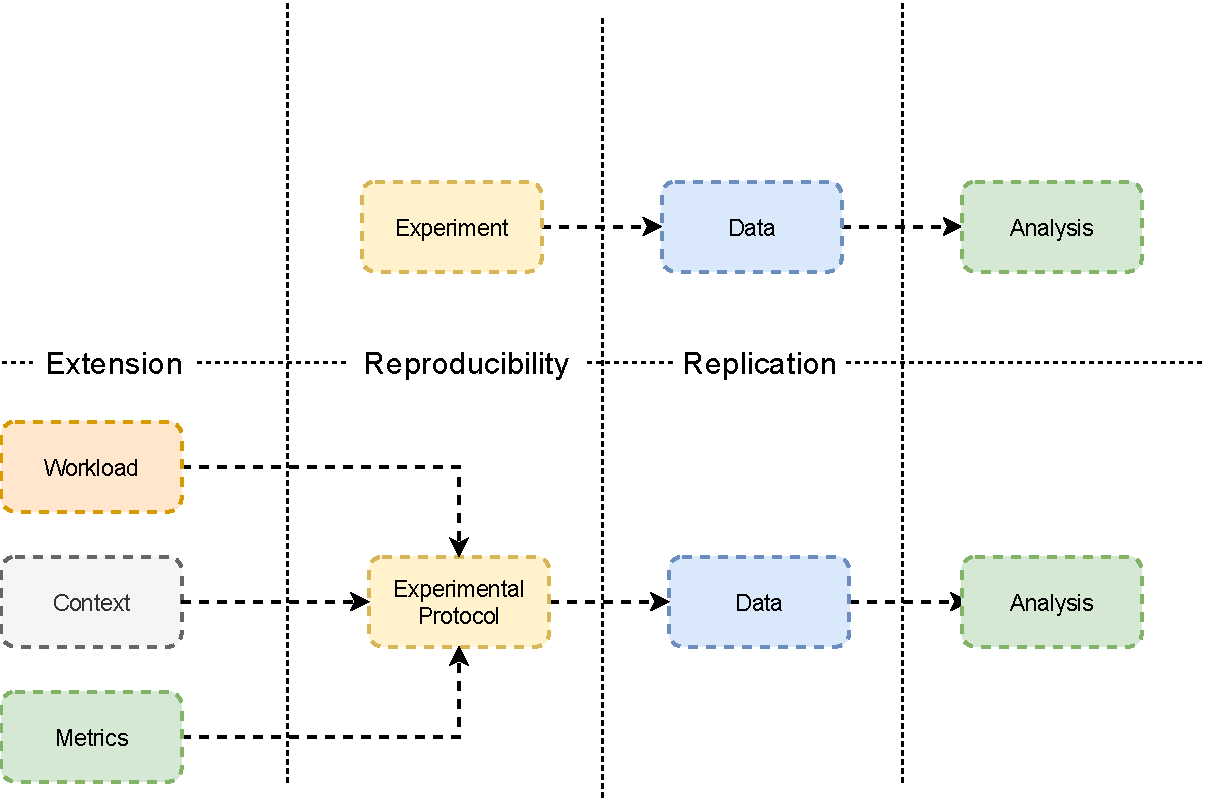
\includegraphics[width=.9\linewidth]{imgs/benchmarkingprotocol}}
%     \caption{Benchmarking protocol}\label{fig:benchmarkingprotocol}
% \end{figure}

later in this chapter we will discuss each aspect of those interfaces 


\section{Reproducibility in Benchmarking}
As discussed in the previous section, the candidates should not be related to the experiment, all they need to know is the interface of the workload.
This section thus discusses different ways to enforce the reproducibility of experiment by comparing different ways to encapsulate the systems-under-test.

\subsection{Virtual Machines}
First option should be using \emph{Virtual Machines} (VM), which gives researchers the freedom to choose the most appropriate tools, software and operating system that they are the most comfortable with, without paying the price to change the actual working environment, which will give them eventually more control over the dependencies and the execution environment.
Moreover, using a VM addresses the \emph{replication crisis} thanks to the virtual images, as even the most complex architecture can be reproduced easily by instantiating a copy of the image.
Since the virtual machines are agnostic to the host architecture, researchers will not have to worry about where and how their experiments are replicated, because they have already setup the execution environment.
Another advantage of VM is the snapshot mechanism, as it allows researchers to create backups and revert some changes with simple clicks. 
Last but not least, thanks to the isolation, virtual machines push the reproducibility further by allowing the future usages to see all the variables---controlled and uncontrolled---and do other analysis without dealing with any dependencies.
In his paper~\cite{howe_virtual_2012}, Bill Howe lists the benefits of using VM in researchers experiments, including the economical impact and cultural limitation to a such approach.
In particular, VM allow them to have control over the resources, the dependencies, and the execution environment.
Moreover, thanks to snapshots, deploying a software is easily achieved by instantiating a copy of that image.
However, this choice comes with a certain cost.
Because of the hypervisor, software will build on two kernels---the virtual machine (guest) one and the host machine one---which will provide a noticeable overhead, and will impact the performances of the system-under-test.
Therefore, we cannot use VM for experiments that are related to performance.
Another limitation of VM is the the isolation.
While this feature prevents the experimental environment from any undesirable interference from the outside world, this interaction may be required---especially when the experiment is dependent to an external part, such as sensors.
For energy measurements, one tend to use hardware power~meters, which will make it difficult to support VM in such a case.

% introduction of docker 
\subsection{Containers}
Another solution would be using something that allows us to benefit from the isolation of the host OS, while easing of replication proposed by VM, and the direct interaction with the hardware that the classical method give.
Containers offer such an advantage, while ensuring the isolation and the ease of replication for application.

Figure~\ref{environement:virtualization_technique} explains the differences in architecture between the types of virtualization and container technologies:
\begin{itemize}
    \item \textsf{Type\,1} runs directly on the hardware, it is mainly used by the cloud providers where there is no host OS, but just VM, use the open-source Xen or VMware ESX hypervisors to be executed;
    \item \textsf{Type\,2} runs over the host OS, mostly used for personal computers.
    VMware server and virtualBox are popular examples of this type, and most of the researchers experimentation are run with this type. However, due to the 2 OS, the applications tend to be slower.
    \item \textsf{Containers}. Instead of its own kernel, containers use the host kernel to run their OS, which makes them lighter, faster and use the full potential of hardware.
    For this category, one can cite \emph{Docker}, \emph{Linux LXC}, or \emph{LXD}~\cite{abuabdo_virtualization_2019}.
\end{itemize}
%  TODO Rephrase so i include it before VMs+ add links to the technologie

\begin{figure}
    \center{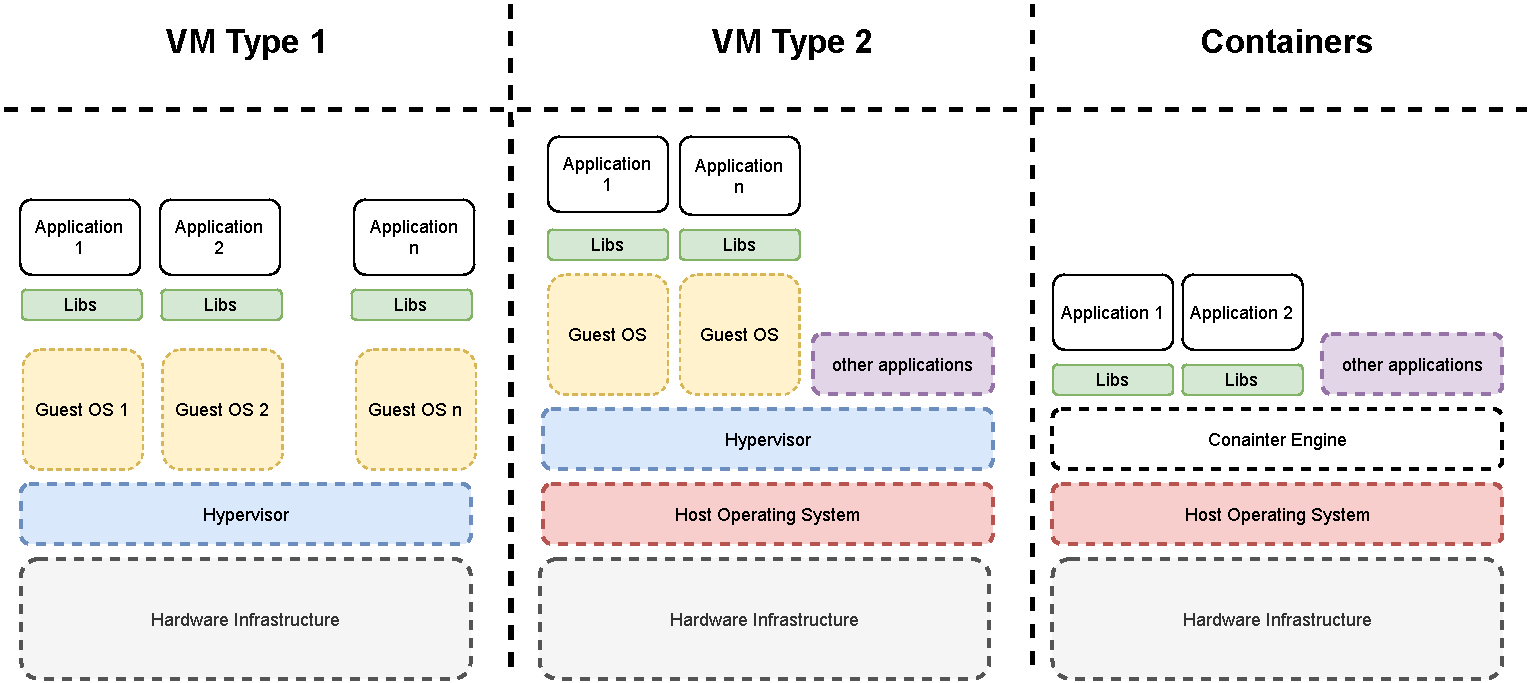
\includegraphics[width=1\linewidth]{imgs/virtualization_techniques}}
    \caption{Different Methods of Virtualization}\label{environement:virtualization_technique}
\end{figure}


\subsection{Docker Vs. Virtual Machine}
Despite the fact that \textsf{Type\,1} is more performant than \textsf{Type\,2}, the second one is the most used in research, as most researchers tend to conduct their experiments in their own machine.
In the other hand, Docker is the most famous container technology.
In our case, we are more prone to promote Docker for two reasons:
\begin{enumerate}
    \item we need a lightweight orchestrator to limit the overhead on energy consumption of our tests, as prior work mentioned [cite Morabito (2015) and van Kessel et al. (2016)],
          % cite Power efficiency of hypervisor-based virtuali- zation versus container-based virtualization. University of Amsterdam.
    \item as we are using hardware sensors to measure the energy consumption, we need to interact with the host OS.
\end{enumerate}

Special notice to \href{https://github.com/powerapi-ng/virtualwatts}{virtualwatts}. A framework that allows us to retireve the energy consumption of a virtual machine.
%%%%% THINGS TO ADD : 
%% -------------- Dont think so 
% the impact of docker on the reprodudicibility 
% Limits of docker 
% The docker files and the clarification of the methodology 


\subsection{Docker \& Energy}
Now that we have chosen to go with the containers technology to encapsulate our tests.
What would be the impact of this solution on the energy consumption of our tests.

Based on the studies of \cite{santos2018does}, who analysed the impact of adding the Docker layer on the energy consumption.
In their experiment, Eddie Antonio~\emph{et~ al.} run multiple benchmarks with and without Ddocker. 
They compared the resulting energy consumption and execution time.
The first step was to see the impact of Docker deamon, while there is no work, to observe the impact of the orchestrator.
Then, they conduct their experiments with the following benchmarks:
\begin{itemize}
    \item Wordpress,
    \item Reddis,
    \item PostgreSQL.
\end{itemize}

The following figures represents the energy consumption of the system-under-test while it is idle.
As one can observe in Figure~\ref{fig:docker_idle}, Docker brings an overhead of around $1,000$ Joules.

\begin{figure}
    \center{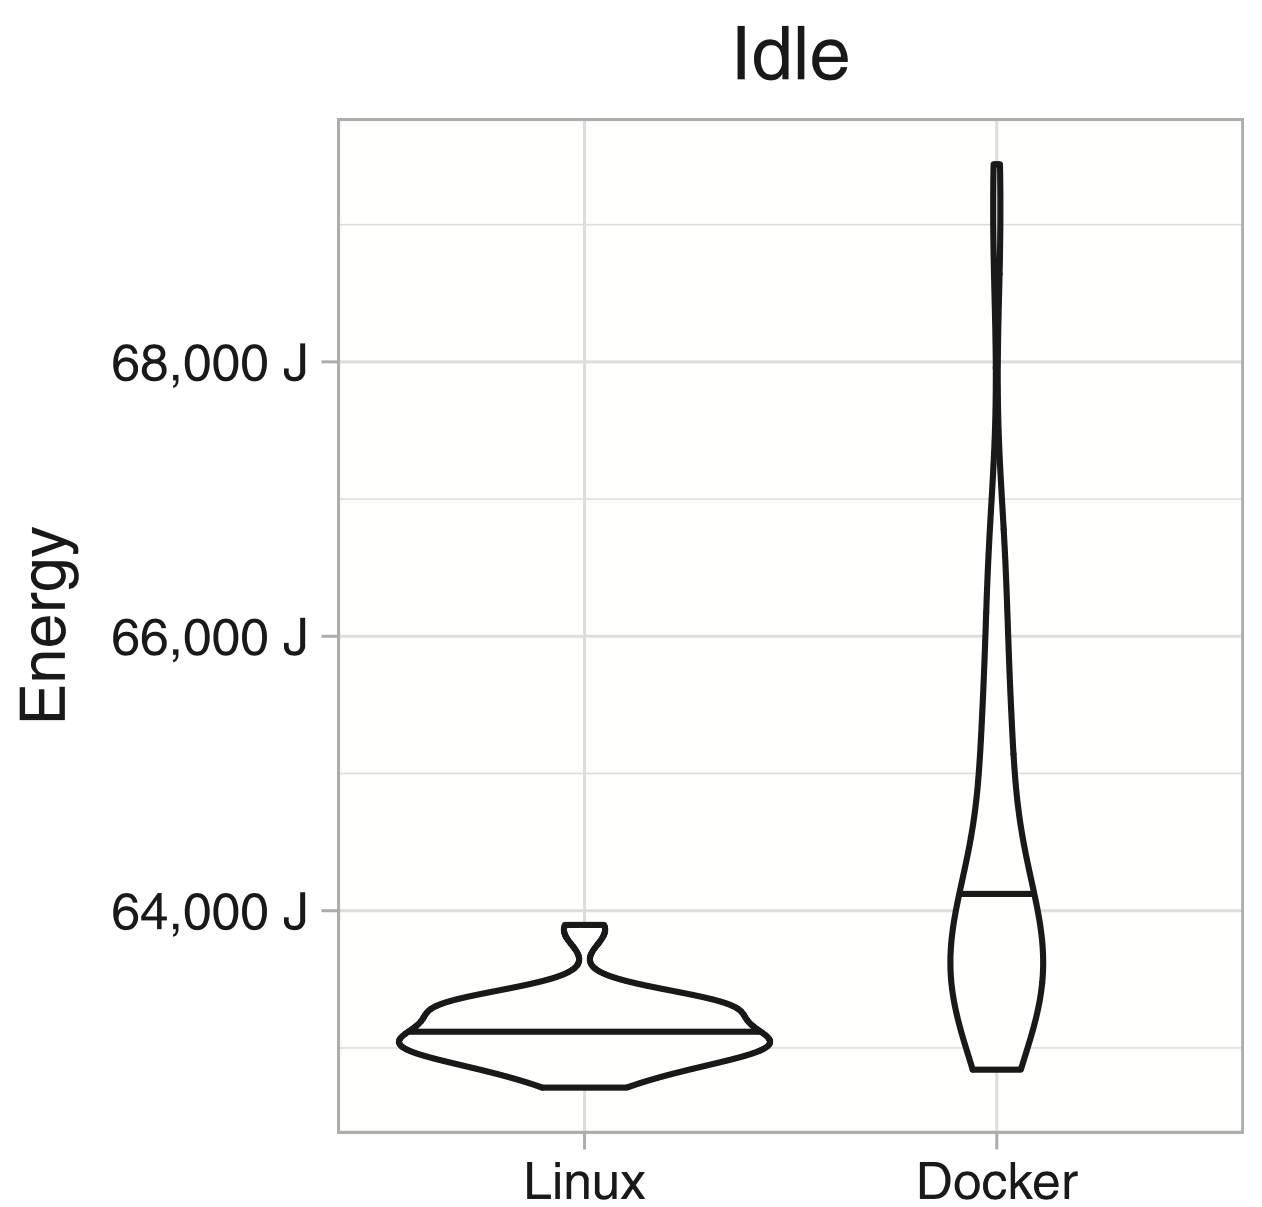
\includegraphics[width=.5\linewidth]{imgs/docker_vs_vm_energy_paper/idle_energy}}
    \caption{energy consumption of Idle system with and without docker \cite{santos2018does}}\label{fig:docker_idle}
\end{figure}

In the other hand, as one can see in Figure~\ref{fig:docker_reddis}.
Docker increased the execution time of the benchmark by 50 seconds, hence increasing the energy consumption.
The authors reported that this overhead is mostly due to the Docker deamon and not the fact that the application is in a container.
Moreover, they estimated the cost of this extra energy and it was less than 0.15\$ in the worst case, which is non-significant compared to the benefits that Docker brings for isolation and reproducibility.

To summarize, Docker-based software tends to consume more energy, because mainly they take more time to be executed.
The average power consumption is higher with only \textbf{2\,Watts}, due to the execution of the Docker deamon.
This overhead can reach up to 5\% for IO-intensive application, but it is merely noticeable when it comes to CPU- or DRMA-intesive workloads.

\begin{figure}
    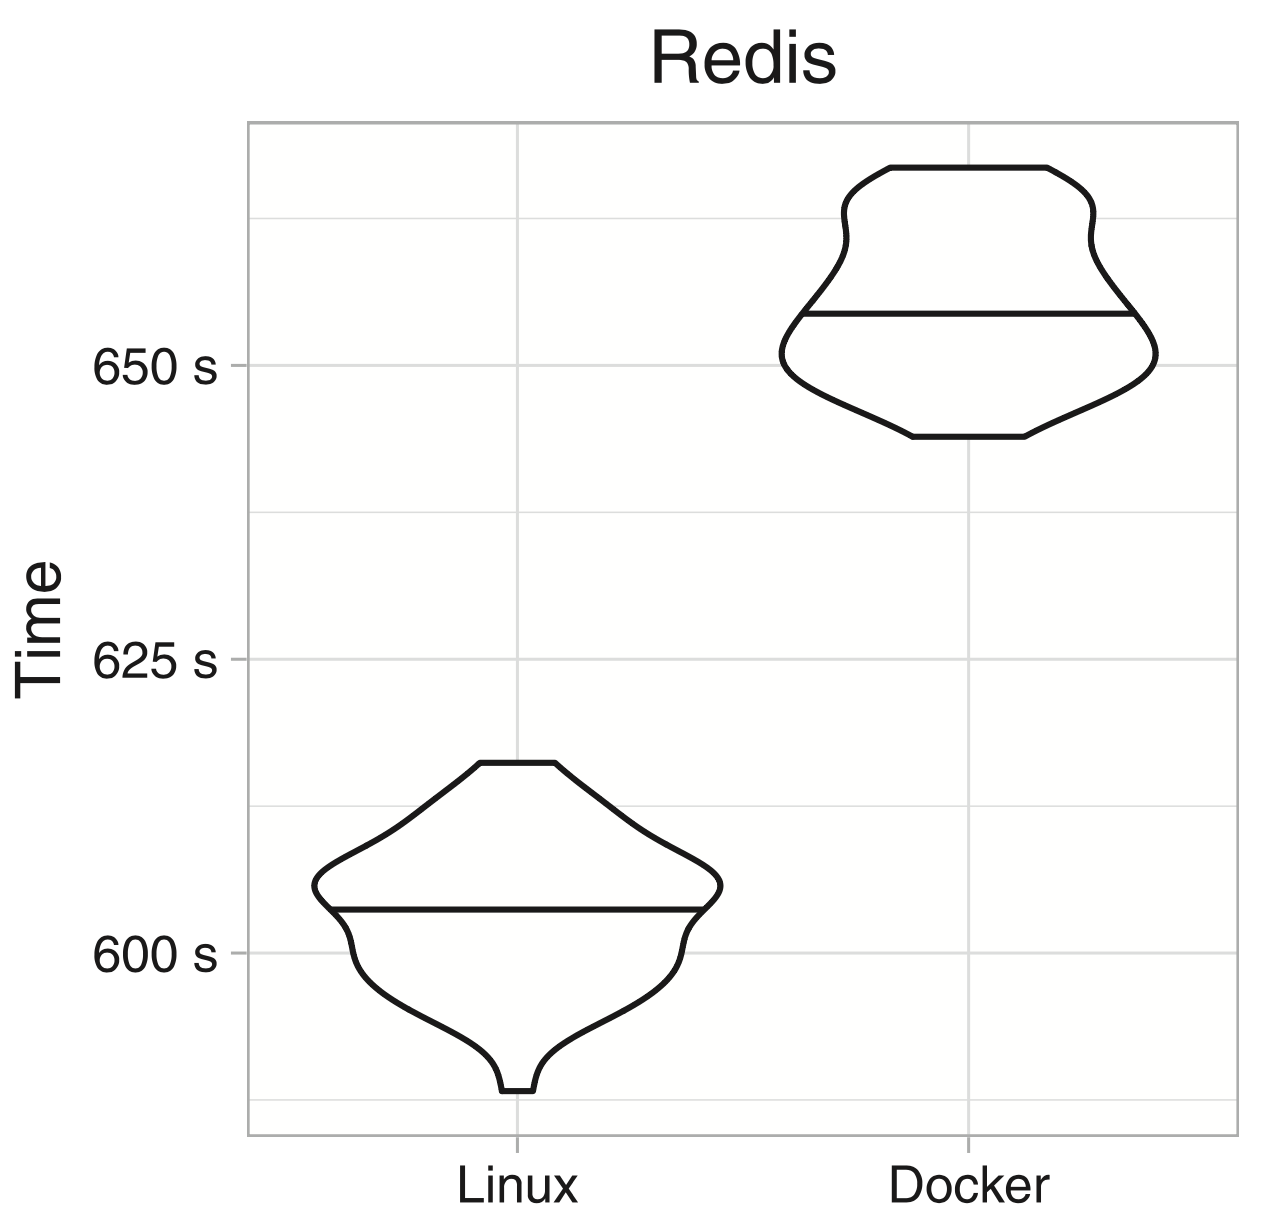
\includegraphics[width=.5\linewidth]{imgs/docker_vs_vm_energy_paper/reddis_time}
    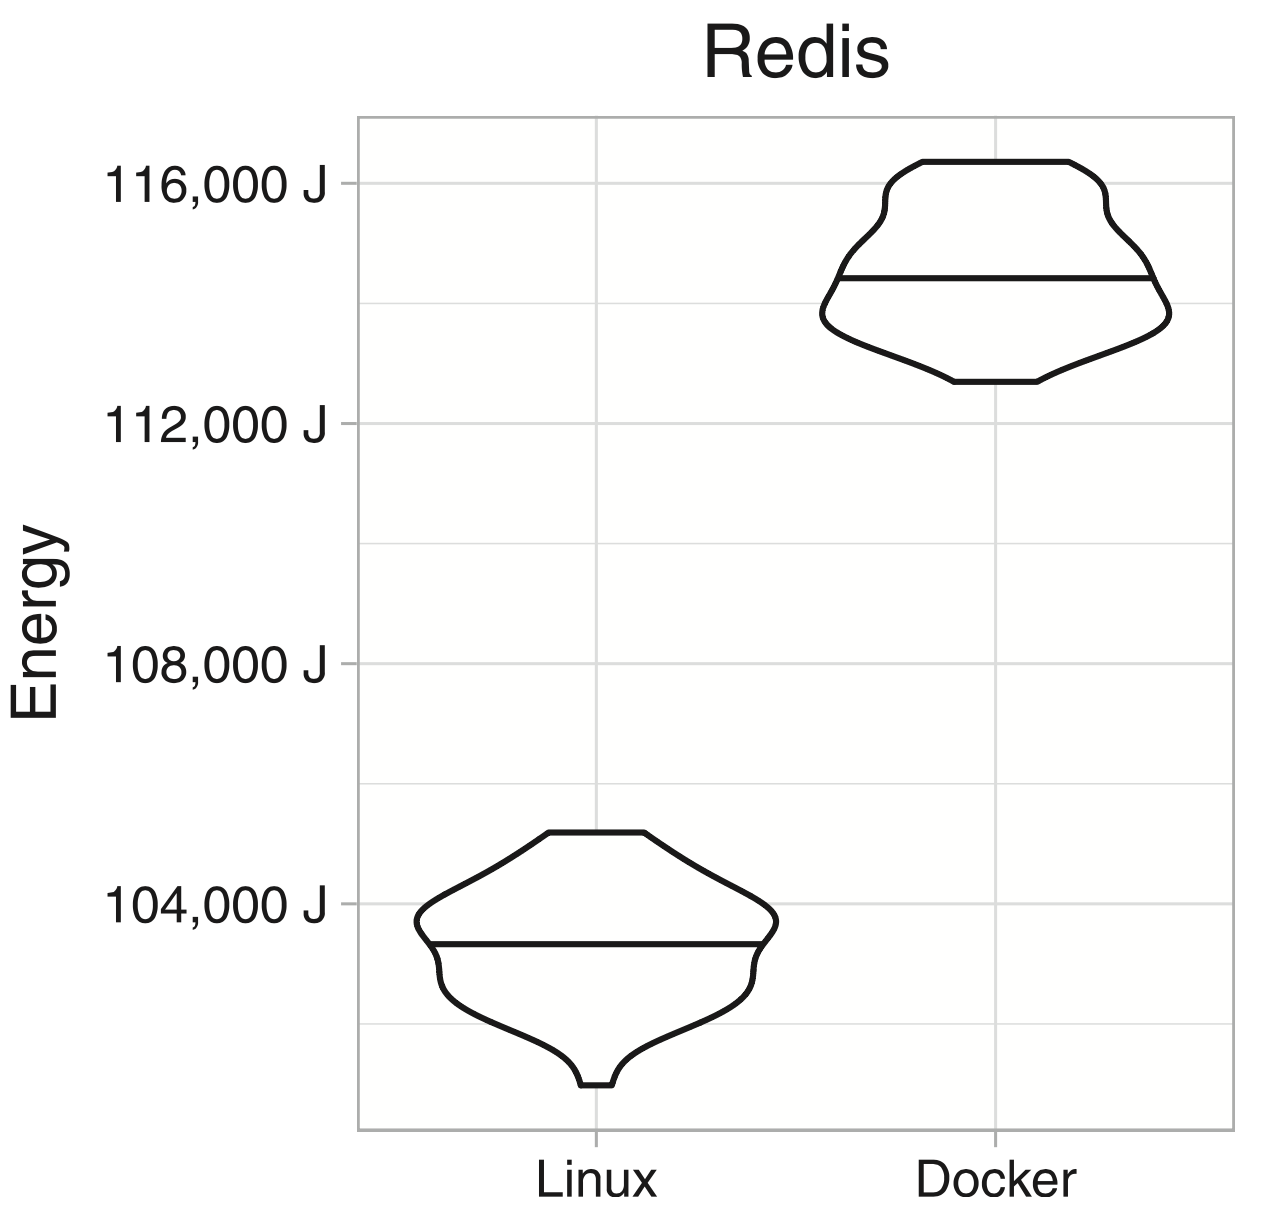
\includegraphics[width=.5\linewidth]{imgs/docker_vs_vm_energy_paper/reddis_energy}
    \caption{Execution time \& energy consumption of Redis with and without Docker~\cite{santos2018does}}\label{fig:docker_reddis}
\end{figure}


\subsection{Docker \& Accuracy}
As the state of the art assesses the impact of Docker on the energy consumption, one can also consider its impact on accuracy.
In other words:\\
\textbf{RQ:} does Docker affect the energy variation of the experiments? %La RQ n'est pas lié au reste du paragraphe, non ?

To answer this question we conducted a preliminary experiment by running the same benchmarks \textsf{LU}, \textsf{CG} and \textsf{EP} in a Docker container and a flat binary format on 3 nodes of the cluster \textsf{Dahu} to assess if Docker induces an additional variation.
Figure~\ref{fig:docker} reports that this is not the case, as the energy consumption variation does not get noticeably affected by Docker while running a same compiled version of the benchmarks at 5\,\%, 50\,\% and 100\,\% workloads.
In fact, while Docker increases the energy consumption due to the extra layer it implements~\cite{eddie_antonio_santos_how}, it does not noticeably affect the energy variation.
The \emph{standard deviation} (STD) is even slightly smaller ($STD_{Docker}=192 mJ$,$STD_{Binary}=207 mJ$), taking into account the measurements errors and the OS activity.

\begin{figure}
    \center{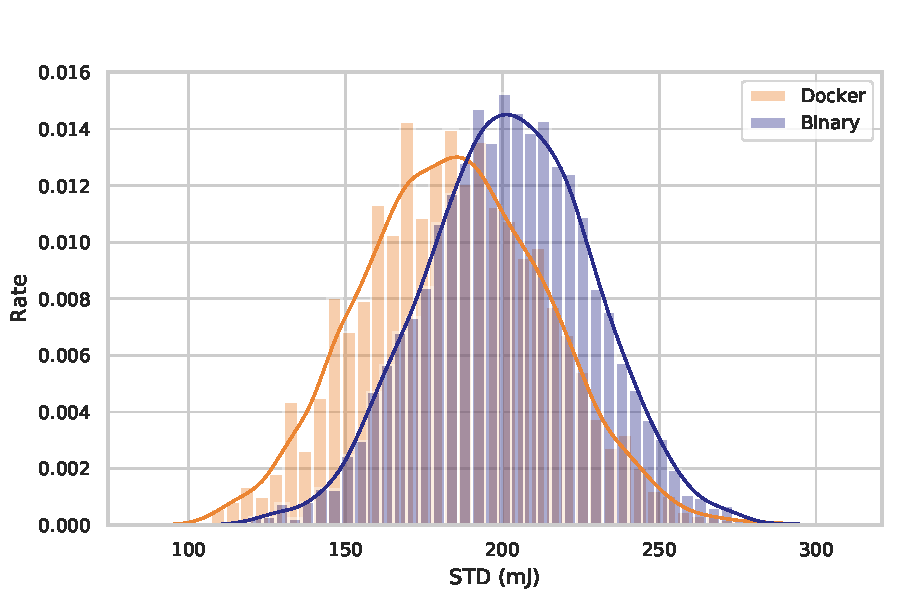
\includegraphics[width=.9\linewidth]{imgs/docvsbin}}
    \caption{Comparing the variation of binary and Docker versions of aggregated \textsf{LU}, \textsf{CG} and \textsf{EP} benchmarks}\label{fig:docker}
\end{figure}